\documentclass[11pt,a4paper]{article}
\usepackage[utf8]{inputenc}
\usepackage[T1]{fontenc}
\usepackage{lmodern}
\usepackage[margin=2.5cm]{geometry}
\usepackage{graphicx}
\usepackage{booktabs}
\usepackage{amsmath,amssymb}
\usepackage{microtype}
\usepackage{float}
\usepackage{caption}
\usepackage{xcolor}
\usepackage[colorlinks=true,linkcolor=blue!50!black,citecolor=blue!50!black,urlcolor=blue!50!black]{hyperref}
\graphicspath{{figures/}}
\captionsetup{font=small,labelfont=bf}

\title{\textbf{Same Words, Different Bets}\\[2pt]
\large Lexicons, Static Embeddings and Contextual Pre-training for Sentiment Classification\\ under Scarce Labels and Ambiguity}
\author{Project report}
\date{\today}

\setlength{\emergencystretch}{3em}
\begin{document}
\maketitle

\begin{abstract}
Everyone agrees that pre-trained transformers are powerful; far fewer studies ask how much pre-training is enough, what else can be done with the same text, and how models behave on ambiguous inputs.
We study binary sentiment classification (SST-2) with scarce labels (100--6\,920) on a CPU, comparing model families under one protocol: a sentiment lexicon that uses no task labels, word and character n-gram TF-IDF models,
static word embeddings (word2vec, fastText) trained on the same 1.2\,M unlabeled words, a 1.17\,M-parameter BERT trained from scratch or after 13 minutes of masked-language-model (MLM) pre-training on those words, and public compact checkpoints (BERT-Tiny, DistilBERT).
Beyond accuracy we measure robustness (typos, word deletion, out-of-domain reviews), calibration, and ``ambiguity-awareness'' using the fine-grained SST-5 labels as a polarity-strength proxy, cross-model consensus difficulty and contrast markers.
\textbf{Findings.} (i) Small-scale MLM pre-training did \emph{not} help ($-0.3$ to $-4.5$ points vs.\ random initialisation), and its deficit sits mainly on \emph{strongly polar} sentences ($-4.7$ [$-7.2$,$-2.2$] vs.\ $-1.3$ [$-3.4$,$+0.8$] on weak-polarity sentences at $n{=}1000$; strong$-$weak difference $-3.5$ [$-6.7$,$-0.3$]).
(ii) The best way to use the \emph{same unlabeled text} depends on the label budget: fastText embeddings are the highest-scoring model at 100--300 labels and beat MLM at $n{=}1000$ ($70.2\%$ vs.\ $65.7\%$), but plateau at $71.2\%$ while the transformers reach $77.5$--$78.5\%$ at $n{=}6920$.
(iii) TF-IDF variants are the strongest from-scratch models from 1\,000 labels on; character n-grams are the most typo-robust; the VADER lexicon reaches $69.4\%$ with zero task labels, worth about 840 TF-IDF labels.
(iv) Transformers trained on few labels are badly overconfident (ECE $22.9$--$25.6\%$ vs.\ $3.1$--$6.4\%$ at $n{=}1000$) and no model's confidence tracks polarity strength well (ambiguity AUROC $\le0.62$; pre-training does not improve it).
(v) Public checkpoints show that pre-training \emph{does} pay off at scale: BERT-Tiny, with the same depth and width as ours, reaches $75.0\%$ at $n{=}1000$, and DistilBERT $86.5\%$ and $90.4\%$.
Our negative result is therefore about scale (1.2\,M words, 13 CPU-minutes), not about pre-training in general.
(vi) Extending the study to two more domains -- Financial PhraseBank (finance news, real annotator-agreement tiers) and Twitter Airline Sentiment (social media, real crowd-worker confidence) -- confirms the pattern: fastText beats MLM pre-training at low labels in airline too ($+3.2$ points [$+2.3,+4.1$] at $n{=}100$), and at full data all three families (TF-IDF, random-init, +MLM) become statistically indistinguishable in both new domains, unlike SST-2 where TF-IDF keeps a significant edge. A cross-domain transfer matrix shows every model loses 15--60 points when tested on a different domain, with TF-IDF (62.7\% movies$\to$finance) transferring better than either tiny transformer (51.8--54.1\%).
\end{abstract}

\section{Introduction}
Pre-trained transformers \cite{devlin2019bert} dominate NLP benchmarks, but practitioners who need models that run locally, with little memory and little labeled data, often turn to compact variants
\cite{turc2019well,sanh2019distilbert,jiao2020tinybert,wang2020minilm}. Those models are pre-trained or distilled with very large corpora and compute. It is much less clear whether the pre-training recipe itself,
applied at laptop scale, still pays off, whether cheaper ways of exploiting the same unlabeled text (static embeddings, lexicons) are competitive, and whether pre-training changes \emph{where} a model makes its mistakes.
TF-IDF linear models remain strong sentiment baselines \cite{wang2012baselines}. This project is a controlled, fully reproducible CPU-scale study addressing seven research questions:

\begin{description}
\item[RQ1 (data efficiency)] Does MLM pre-training on a small unlabeled in-domain corpus beat random initialisation and TF-IDF baselines when labels are scarce?
\item[RQ2 (robustness)] How do the models cope with typos, dropped words and domain shift?
\item[RQ3 (amount of pre-training)] How do downstream and linear-probe accuracy evolve with the number of pre-training steps?
\item[RQ4 (efficiency)] What are model size, CPU latency and throughput, and what does INT8 quantization change?
\item[RQ5 (public checkpoints)] How far do publicly available pre-trained compact models move the picture?
\item[RQ6 (model families)] Which way of using the same unlabeled text (none, static embeddings, contextual MLM) works best at which label budget, and how do sparse, lexicon and neural families compare?
\item[RQ7 (ambiguity)] Where do errors concentrate on ambiguous sentences, does pre-training change that, and do models' confidences reflect ambiguity?
\item[RQ8 (cross-domain generalisation)] Do the RQ1/RQ6 findings hold in other domains, and how well does a model trained on one domain transfer to another?
\end{description}

\section{Related Work}
BERT \cite{devlin2019bert} popularised MLM pre-training. Turc et al.\ \cite{turc2019well} study pre-trained compact
BERTs (including the 2-layer/128-dim ``BERT-Tiny'') and show pre-training plus distillation is essential when models are
small; DistilBERT \cite{sanh2019distilbert}, TinyBERT \cite{jiao2020tinybert} and MiniLM \cite{wang2020minilm} compress larger
teachers. Gururangan et al.\ \cite{gururangan2020dont} show that continued in-domain pre-training helps
large models. Linear bag-of-n-gram models with TF-IDF-style weighting remain strong for sentiment \cite{wang2012baselines}.
Post-training dynamic quantization for BERT was explored e.g.\ by Zafrir et al.\ \cite{zafrir2019q8bert}. Our study
differs in scale: the pre-training corpus is several orders of magnitude smaller than that of public checkpoints.

\paragraph{Static embeddings, lexicons and classical models.} Word2vec \cite{mikolov2013efficient,mikolov2013distributed} and fastText \cite{bojanowski2017enriching} learn static word vectors from unlabeled text, the latter with sub-word information;
VADER \cite{hutto2014vader} is a rule-based lexicon model that needs no training labels; linear SVMs \cite{cortes1995support} and character n-gram features are standard robust baselines. We include them because they consume the same unlabeled text (or none) as contextual pre-training.

\paragraph{Ambiguity, disagreement and calibration.} Human annotators disagree systematically on many items \cite{pavlick2019inherent,nie2020can,plank2022problem}, evaluation should therefore not treat every label as unambiguous \cite{baan2022stop}, and
training dynamics can single out ``ambiguous'' examples \cite{swayamdipta2020dataset}. Language models are also weak at handling ambiguity explicitly \cite{liu2023afraid}. Modern networks tend to be over-confident \cite{guo2017calibration}, although pre-trained transformers are often better calibrated in-domain than non-pre-trained ones \cite{desai2020calibration}.
We do not propose a new ambiguity method; we use a graded human-derived signal (polarity strength) together with cross-model consensus and linguistic markers to ask how model families and pre-training scale behave on ambiguous inputs.

\section{Experimental Setup}
\subsection{Data}
\textbf{SST-2} \cite{socher2013recursive}: 6\,920 / 872 / 1\,821 sentences (train / dev / test), binary polarity, lower-cased and tokenised, obtained from a public GitHub mirror.
\textbf{NLTK \texttt{movie\_reviews}} \cite{pang2004sentimental}: 2\,000 IMDb reviews (1\,000 pos.\ / 1\,000 neg.), split \emph{by document}:
1\,600 reviews (1.19\,M words) are used \emph{without labels} for MLM pre-training; 400 reviews are held out and used only as an \textbf{out-of-domain (OOD)} test set.
Each held-out review is cut into up to eight 40-word chunks; chunk probabilities are averaged and the review is classified by the mean.
SST-2 and IMDb differ in length and style (short critic snippets vs.\ long user reviews).

Labeled budgets are $n\in\{100,300,1000,3000,6920\}$ sentences (stratified subsets; the same subset for every model given a seed; seeds $\{0,1,2\}$).
At $n=6920$ the training set is identical across seeds, so seed variation reflects only initialisation and data order (and is exactly zero for the deterministic TF-IDF models).

\textbf{Two more domains (RQ8).} \textbf{Financial PhraseBank} \cite{malo2014good} (CC-BY-NC-SA 3.0): finance news headlines with \emph{real} annotator-agreement tiers (not a proxy) -- 50--65\%, 66--99\%, 100\% agreement, verified by cross-checking three independent mirrors (zero label mismatches on 2\,259 overlapping sentences). Neutral sentences dropped, giving 1\,966 binary sentences (1\,377 / 196 / 394 train/dev/test, stratified, seed 42); budgets $n\in\{50,100,300,700,1377\}$.
\textbf{Twitter US Airline Sentiment} (CrowdFlower/Kaggle origin): tweets with a \emph{real} per-tweet crowd-worker confidence score (continuous, 0.335--1.0). Neutral dropped, giving 11\,541 binary tweets (8\,125 / 1\,009 / 2\,407 train/dev/test); budgets $n\in\{100,300,1000,3000,8125\}$.
Every model trained on one domain is also evaluated, zero-shot, on the other two domains' test sets (cross-domain transfer), at no extra training cost. \emph{Tiny-BERT +MLM} reuses the \emph{same} movie-review-pretrained checkpoint on every domain -- deliberately, to test whether pre-training on one domain transfers to fine-tuning on another; static embeddings and TF-IDF are refit fresh on each domain's own text. The pre-training-length ablation (RQ3) is sst2-only.

\subsection{Models}
\begin{itemize}
\item \textbf{Tiny-BERT (ours)}: BERT encoder with 2 layers, hidden size 128, 2 heads, feed-forward size 512, a 6\,000-token WordPiece vocabulary trained on the pre-training corpus, maximum length 64; 1.17\,M parameters in total. Head: masked mean pooling $\rightarrow$ dropout 0.1 $\rightarrow$ linear.
\emph{Random init} is this network fine-tuned from random weights; \emph{+MLM} is the same network after MLM pre-training.
\item \textbf{TF-IDF + LogReg / NaiveBayes}: word 1--2-gram TF-IDF (sublinear tf); regularisation $C\in\{0.3,1,3,10,30\}$ or $\alpha\in\{0.1,0.3,1\}$ chosen on dev.
\item \textbf{Public checkpoints} (RQ5, run through exactly the same fine-tuning code, head and evaluation sets): \texttt{google/bert\_uncased\_L-2\_H-128\_A-2} (``BERT-Tiny'', 4.4\,M parameters; the same 2-layer/128-dimensional transformer stack as ours, but a 30\,522-token vocabulary) and \texttt{distilbert-base-uncased} (66.4\,M parameters). Learning rates were $3\times10^{-4}$ and $5\times10^{-5}$ respectively and were \emph{not} tuned.
\item \textbf{Other model families} (RQ6; identical subsets, dev-based selection and evaluation sets): (a) the \textbf{VADER} sentiment lexicon \cite{hutto2014vader}, rule-based, with no task labels (the sign of its compound score); (b) word 1--2-gram TF-IDF + \textbf{linear SVM} \cite{cortes1995support}; (c) \textbf{character} 2--5-gram (word-boundary) TF-IDF + logistic regression; (d) skip-gram \textbf{word2vec} and (e) \textbf{fastText} (100 dimensions, 5 epochs, both trained on the \emph{same 1.2\,M unlabeled words} as our MLM) with averaged word vectors + logistic regression. Regularisation is chosen on dev; embedding hyper-parameters were not tuned.
\end{itemize}

\subsection{MLM pre-training}
Corpus text is tokenised, concatenated into blocks of 62 wordpieces plus \texttt{[CLS]}/\texttt{[SEP]} (22\,982 training and 1\,209 held-out blocks; 1.47\,M tokens per epoch).
Standard BERT masking is used (15\% of tokens: 80\% \texttt{[MASK]}, 10\% random, 10\% unchanged), with the vocabulary projection computed only at masked positions.
Optimiser: AdamW, learning rate $10^{-3}$, 6\% warm-up then linear decay, batch 128, weight decay 0.01, $\beta_2{=}0.98$, gradient clipping 1.0, \textbf{no dropout}, 5\,000 steps ($\approx$28 epochs, 13 minutes).
During development, a first attempt with learning rate $2\times10^{-3}$ and dropout 0.1, and short schedules with learning rates $5\times10^{-4}$ and $10^{-3}$, stayed on the unigram plateau (loss $\approx6.15$);
the final recipe (no dropout, lr $10^{-3}$, 5\,000 steps) leaves the plateau after roughly 1\,500 steps (Fig.~\ref{fig:pretrain}). Tiny-scale pre-training is thus sensitive to the recipe.

\begin{figure}[t]
\centering
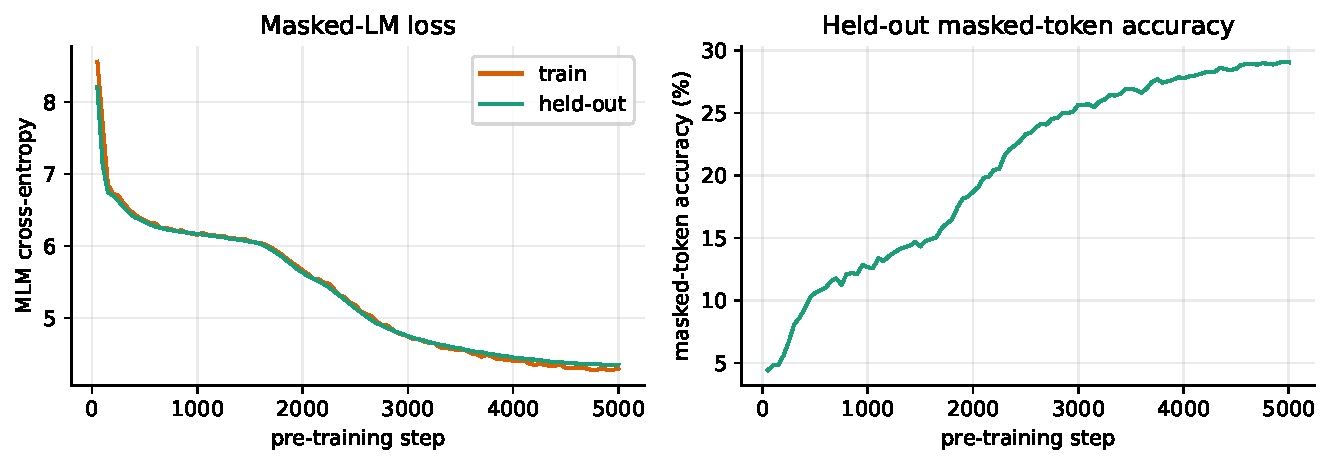
\includegraphics[width=0.95\linewidth]{fig_pretrain.pdf}
\caption{MLM pre-training. Held-out loss falls from 8.2 to 4.35 (perplexity 77); masked-token accuracy reaches 29.1\%. Loss stays near the unigram entropy (about 6.1--6.2) for roughly the first 1\,500 steps.}
\label{fig:pretrain}
\end{figure}

\subsection{Fine-tuning protocol}
AdamW (weight decay 0.01), batch 32, 10\% warm-up then linear decay, a number of epochs equal to $600/(\text{steps per epoch})$ rounded up and clipped to $[5,30]$,, dropout 0.1; the epoch with the best dev accuracy is kept.
The learning rate for each of our two initialisations was selected in a pilot on dev accuracy (five values from $2\times10^{-4}$ to $4\times10^{-3}$; seed 0, $n\in\{300,3000\}$; Table~\ref{tab:pilot}); the pilot chose $2\times10^{-4}$ for both (the lowest value in the grid).
The test sets were used only for final evaluation.

\subsection{Perturbations, metrics and environment}\label{sec:setupstats}
Robustness is measured on the SST-2 test set perturbed by (a) swapping two adjacent inner characters in 10\% / 30\% of words (\emph{typos}), (b) deleting 20\% / 40\% of words (\emph{word-drop}); perturbed sets are generated once with a fixed seed so all models see identical inputs.
We report accuracy (macro-F1 is in \texttt{results/all\_runs.csv}), mean $\pm$ standard deviation over 3 seeds, and paired bootstrap confidence intervals (2\,000 resamples of test sentences, pooled over seeds).
All experiments ran on the CPU of a single laptop with Python 3.13, PyTorch 2.14 and Transformers 5.17.

\subsection{Ambiguity signals and metrics}\label{sec:ambsetup}
We use three complementary signals for the 1\,821 SST-2 test sentences.
\textbf{(A1) Polarity strength} from the fine-grained SST-5 labels \cite{socher2013recursive} (all sentences matched, and 100\% are consistent with their binary label): \emph{strong} = very negative or very positive (678 sentences), \emph{weak} = negative or positive but mild, close to neutral (1\,143 sentences, 62.8\%). This is a graded-intensity proxy for ambiguity, \emph{not} annotator disagreement.
\textbf{(A2) Consensus difficulty}: the fraction of the 27 runs of our nine core models that classify a sentence correctly; it checks that A1 is related to what is hard for models.
\textbf{(A3) Linguistic markers}: sentences containing a contrast word (\emph{but, however, although, though, yet, despite, whereas, while}; 337 sentences) or negation (371 sentences).
Per model and label budget we report accuracy on each stratum, mean confidence (maximum class probability), an \emph{ambiguity-awareness} AUROC (how well low confidence identifies weak-polarity sentences; 0.5 = chance), expected calibration error (ECE, 15 bins; only for models with probabilistic outputs), and accuracy on the 50\% most confident predictions.
Differences between models inside a stratum use the paired bootstrap of Section~\ref{sec:setupstats}; an \emph{interaction} interval tests whether a difference is larger on strong than on weak sentences (strata resampled independently).

\section{Results}
\subsection{RQ1: data efficiency}
Table~\ref{tab:main} and Fig.~\ref{fig:curve} (left) show the learning curves. All methods improve monotonically with $n$. At $n=100$ all models are within 2 points of each other.
From $n\ge300$ MLM pre-training is \emph{worse} than random initialisation: $-4.5$, $-2.5$, $-2.3$ points at $n=300,1000,3000$ with 95\% intervals excluding zero (Table~\ref{tab:stats}); at $n=100$ ($-0.3$) and $n=6920$ ($-1.0$) the difference is not resolvable.
TF-IDF is stronger than both transformers from $n\ge1000$ (random init: $-2.2$ to $-2.8$ points; pre-trained: $-3.9$ to $-4.8$ points, intervals exclude zero); at $n=300$ TF-IDF+LogReg still beats the pre-trained model by 4.4 points but ties random init.
NaiveBayes is the best of our models at every budget.

\begin{table}[t]
\centering\small
\caption{SST-2 test accuracy (\%), mean$\pm$std over 3 seeds, as a function of labeled training size $n$.}\label{tab:main}
\resizebox{\linewidth}{!}{\begin{tabular}{lccccc}
\toprule
Model & $n{=}100$ & $n{=}300$ & $n{=}1000$ & $n{=}3000$ & $n{=}6920$ \\
\midrule
TF-IDF + LogReg & 57.9$\pm$1.7 & 63.2$\pm$1.7 & 70.5$\pm$0.7 & 77.5$\pm$1.0 & 81.3$\pm$0.0 \\
TF-IDF + NaiveBayes & 58.6$\pm$1.6 & 64.5$\pm$0.4 & 71.6$\pm$0.7 & 78.6$\pm$0.8 & 81.9$\pm$0.0 \\
Tiny-BERT (random init) & 57.0$\pm$0.7 & 63.2$\pm$0.5 & 68.2$\pm$1.3 & 75.2$\pm$0.3 & 78.5$\pm$0.9 \\
Tiny-BERT (+MLM pre-training) & 56.8$\pm$0.7 & 58.7$\pm$3.8 & 65.7$\pm$0.9 & 72.9$\pm$0.1 & 77.5$\pm$1.1 \\
\bottomrule
\end{tabular}}
\end{table}

\begin{table}[t]
\centering\small
\caption{Paired bootstrap (2000 resamples of the test set, pooled over 3 seeds): accuracy difference in points with 95\% CI. $^*$ = CI excludes 0.}\label{tab:stats}
\resizebox{\linewidth}{!}{\begin{tabular}{lccccc}
\toprule
Comparison & $n{=}100$ & $n{=}300$ & $n{=}1000$ & $n{=}3000$ & $n{=}6920$ \\
\midrule
Tiny +MLM $-$ Tiny random & -0.3 [-2.1, +1.4] & -4.5 [-6.3, -2.8]$^*$ & -2.5 [-4.2, -1.0]$^*$ & -2.3 [-4.0, -0.8]$^*$ & -1.0 [-2.6, +0.5] \\
Tiny +MLM $-$ TF-IDF+LR & -1.1 [-3.1, +0.8] & -4.4 [-6.2, -2.6]$^*$ & -4.8 [-6.7, -2.9]$^*$ & -4.6 [-6.4, -2.7]$^*$ & -3.9 [-5.8, -1.9]$^*$ \\
Tiny random $-$ TF-IDF+LR & -0.9 [-2.4, +0.5] & +0.1 [-1.4, +1.5] & -2.3 [-3.7, -0.8]$^*$ & -2.2 [-3.8, -0.7]$^*$ & -2.8 [-4.5, -1.0]$^*$ \\
\bottomrule
\end{tabular}}
\end{table}


\begin{figure}[t]
\centering
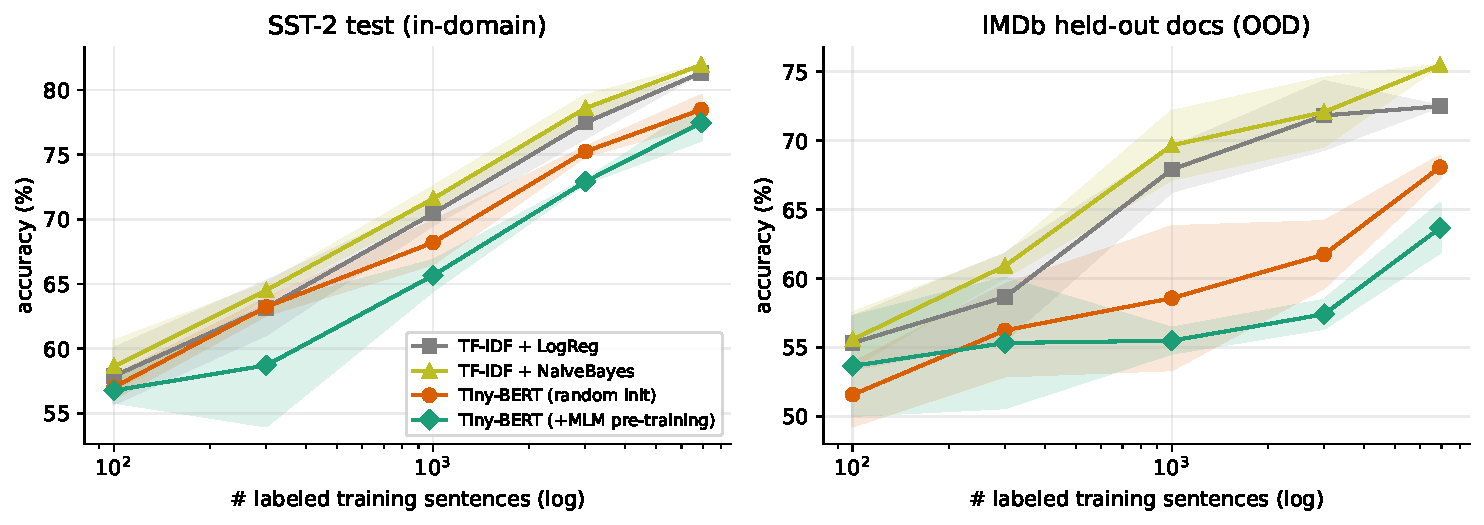
\includegraphics[width=\linewidth]{fig_learning_curve.pdf}
\caption{Learning curves (mean $\pm$ 1 std over 3 seeds). Left: SST-2 test. Right: held-out IMDb reviews (out-of-domain, 400 documents, binomial standard error $\approx2.4$ points).}
\label{fig:curve}
\end{figure}

\subsection{RQ2: robustness and domain shift}
Tables~\ref{tab:robust1000} and~\ref{tab:robust6920} and Fig.~\ref{fig:robust} give accuracy under perturbations. Relative to clean accuracy at $n=6920$ (Table~\ref{tab:drop}), character typos hurt the transformers more than TF-IDF
($-4.9$ random init and $-6.9$ pre-trained vs.\ $-3.8$ / $-2.9$ for TF-IDF LogReg / NaiveBayes at 30\% typos), consistent with WordPiece fragmenting a mis-spelled word into unrelated pieces while TF-IDF simply loses one feature.
Under word-dropping the picture reverses at the mild level (20\%: $-1.6$ and $-0.7$ for the transformers vs.\ $-3.4$ / $-2.9$ for TF-IDF), while at 40\% all models lose 5.6--6.3 points. TF-IDF nevertheless has the highest absolute accuracy under every perturbation.

On the out-of-domain IMDb reviews the transformers trained from our small corpus are clearly behind TF-IDF, and pre-training does not help: at $n=1000$ the pre-trained model reaches $55.5\pm0.7$ vs.\ $58.6\pm4.2$ for random init; at $n=6920$ $63.7\pm1.4$ vs.\ $68.1\pm0.7$; TF-IDF reaches $67.9$--$69.7$ and $72.5$--$75.5$ respectively.
Seed variation on this 400-review set is large (up to 4 points), so small differences should not be over-interpreted, but the gap to TF-IDF (4--14 points) is not noise.

\begin{table}[t]
\centering\small
\caption{Accuracy (\%) under input perturbations and on out-of-domain IMDb documents, models trained on $n=1000$ sentences.}\label{tab:robust1000}
\resizebox{\linewidth}{!}{\begin{tabular}{lcccccc}
\toprule
Model & clean & typos 10\% & typos 30\% & word-drop 20\% & word-drop 40\% & OOD IMDb \\
\midrule
TF-IDF + LogReg & 70.5$\pm$0.7 & 69.7$\pm$0.4 & 68.4$\pm$1.5 & 69.3$\pm$1.0 & 67.2$\pm$1.1 & 67.9$\pm$1.3 \\
TF-IDF + NaiveBayes & 71.6$\pm$0.7 & 70.7$\pm$1.3 & 69.1$\pm$0.1 & 70.7$\pm$1.2 & 68.7$\pm$0.5 & 69.7$\pm$2.0 \\
Tiny-BERT (random init) & 68.2$\pm$1.3 & 67.0$\pm$1.0 & 64.6$\pm$0.3 & 67.2$\pm$1.5 & 64.8$\pm$1.7 & 58.6$\pm$4.2 \\
Tiny-BERT (+MLM pre-training) & 65.7$\pm$0.9 & 64.0$\pm$1.2 & 60.9$\pm$1.2 & 64.7$\pm$0.9 & 62.1$\pm$1.0 & 55.5$\pm$0.7 \\
\bottomrule
\end{tabular}}
\end{table}

\begin{table}[t]
\centering\small
\caption{Accuracy (\%) under input perturbations and on out-of-domain IMDb documents, models trained on $n=6920$ sentences.}\label{tab:robust6920}
\resizebox{\linewidth}{!}{\begin{tabular}{lcccccc}
\toprule
Model & clean & typos 10\% & typos 30\% & word-drop 20\% & word-drop 40\% & OOD IMDb \\
\midrule
TF-IDF + LogReg & 81.3$\pm$0.0 & 80.0$\pm$0.0 & 77.5$\pm$0.0 & 77.9$\pm$0.0 & 75.7$\pm$0.0 & 72.5$\pm$0.0 \\
TF-IDF + NaiveBayes & 81.9$\pm$0.0 & 80.9$\pm$0.0 & 79.1$\pm$0.0 & 79.0$\pm$0.0 & 75.6$\pm$0.0 & 75.5$\pm$0.0 \\
Tiny-BERT (random init) & 78.5$\pm$0.9 & 76.5$\pm$1.0 & 73.6$\pm$0.8 & 77.0$\pm$0.4 & 72.9$\pm$0.4 & 68.1$\pm$0.7 \\
Tiny-BERT (+MLM pre-training) & 77.5$\pm$1.1 & 75.2$\pm$1.7 & 70.6$\pm$1.9 & 76.8$\pm$1.3 & 71.6$\pm$0.7 & 63.7$\pm$1.4 \\
\bottomrule
\end{tabular}}
\end{table}

\begin{table}[t]
\centering\small
\caption{Change in accuracy (percentage points) relative to clean test, full training set.}\label{tab:drop}
\resizebox{\linewidth}{!}{\begin{tabular}{lcccc}
\toprule
Model & typos 10\% & typos 30\% & word-drop 20\% & word-drop 40\% \\
\midrule
TF-IDF + LogReg & -1.4 & -3.8 & -3.4 & -5.6 \\
TF-IDF + NaiveBayes & -1.0 & -2.9 & -2.9 & -6.3 \\
Tiny-BERT (random init) & -2.0 & -4.9 & -1.5 & -5.5 \\
Tiny-BERT (+MLM pre-training) & -2.3 & -6.9 & -0.7 & -5.9 \\
\bottomrule
\end{tabular}}
\end{table}


\begin{figure}[t]
\centering
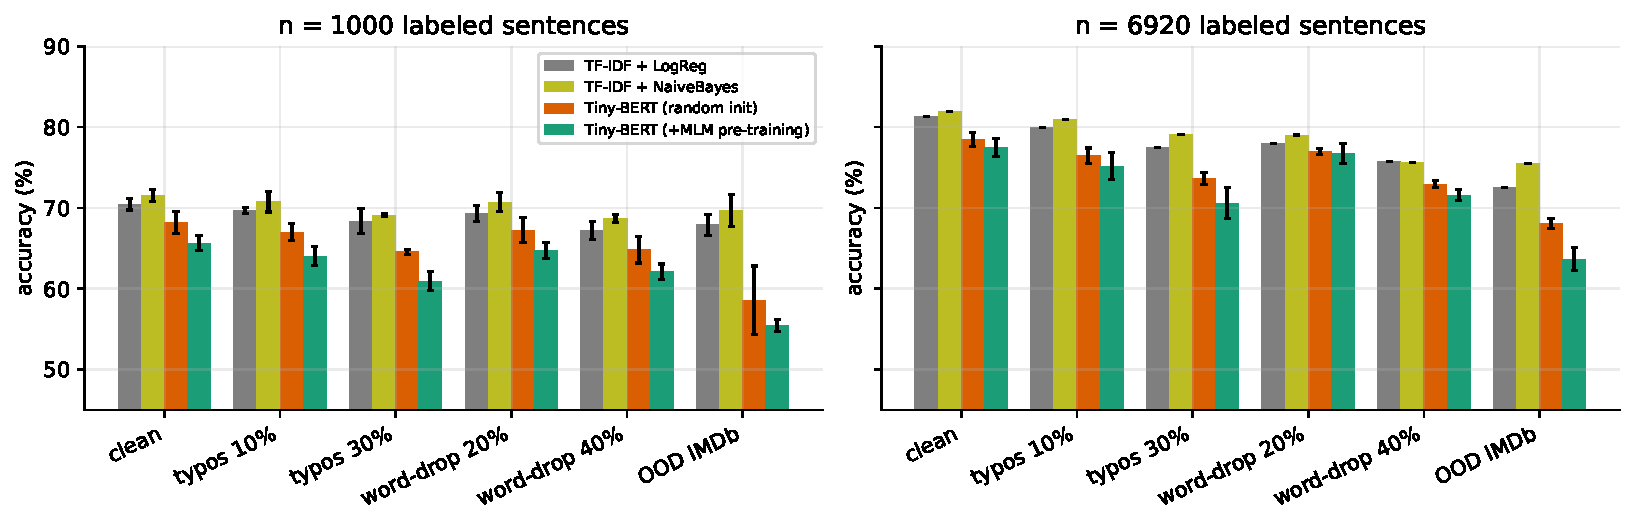
\includegraphics[width=\linewidth]{fig_robustness.pdf}
\caption{Accuracy on clean, perturbed and out-of-domain test data for $n=1000$ (left) and $n=6920$ (right); error bars are 1 std over seeds.}
\label{fig:robust}
\end{figure}

\subsection{RQ3: how much pre-training?}
We fine-tuned ($n=1000$, learning rate $2\times10^{-4}$) checkpoints taken after 0, 100, 300, 1\,000, 2\,500 and 5\,000 MLM steps, and trained a logistic-regression probe on the \emph{frozen} mean-pooled encoder output (Table~\ref{tab:ckpt}, Fig.~\ref{fig:ckpt}).
The frozen-representation probe improves slowly but steadily, from $56.4\pm0.7$ to $59.4\pm1.1$ (+3.0 points), so MLM does inject some sentiment-relevant information, but absolute probe accuracy stays low.
Fine-tuned in-domain accuracy moves the opposite way: it decreases from $69.7\pm0.7$ (step 0, a random initialisation) to $65.7\pm0.9$ at 5\,000 steps (minimum $64.2\pm2.5$ at 1\,000 steps).
OOD accuracy shows no trend ($58.5\pm4.5$ at step 0, $55.5\pm0.7$ at 5\,000). The step-0 checkpoint uses one fixed random initialisation for all three seeds whereas the curve entry draws a new one per seed, so the 1.5-point gap between the step-0 value and the ``random init'' curve entry ($68.2$) indicates the noise floor of comparisons of this size.
These results describe under-trained pre-training (final MLM loss 4.35, masked accuracy 29\%).

\begin{table}[t]
\centering\small
\caption{Effect of the amount of pre-training ($n{=}1000$ labeled sentences, 3 seeds, test accuracy \%).}\label{tab:ckpt}
\resizebox{\linewidth}{!}{\begin{tabular}{rccc}
\toprule
MLM steps & Linear probe & Fine-tuned & Fine-tuned OOD IMDb \\
\midrule
0 & 56.4$\pm$0.7 & 69.7$\pm$0.7 & 58.5$\pm$4.5 \\
100 & 56.9$\pm$1.2 & 69.3$\pm$0.7 & 56.6$\pm$4.8 \\
300 & 56.0$\pm$0.9 & 67.6$\pm$1.3 & 56.8$\pm$4.7 \\
1000 & 58.4$\pm$0.2 & 64.2$\pm$2.5 & 59.0$\pm$2.9 \\
2500 & 59.3$\pm$1.3 & 66.2$\pm$1.1 & 59.7$\pm$3.8 \\
5000 & 59.4$\pm$1.1 & 65.7$\pm$0.9 & 55.5$\pm$0.7 \\
\bottomrule
\end{tabular}}
\end{table}


\begin{figure}[t]
\centering
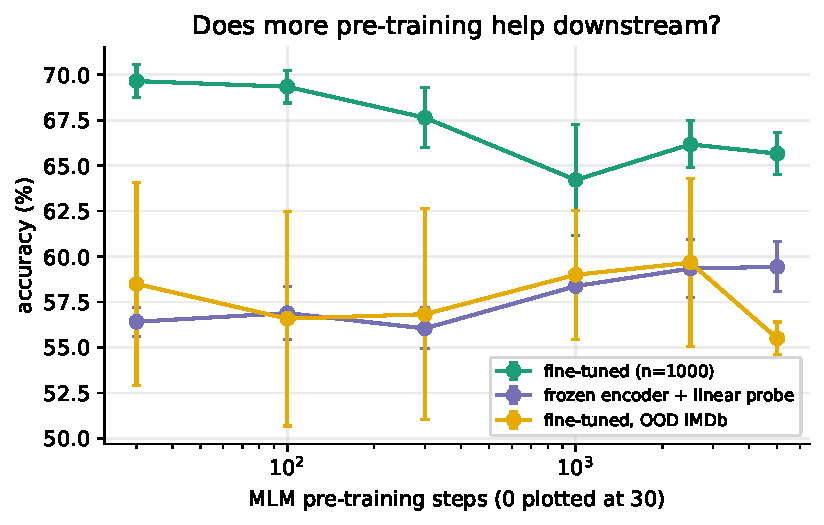
\includegraphics[width=0.62\linewidth]{fig_ckpt.pdf}
\caption{Pre-training length ablation ($n=1000$; mean $\pm$ std over 3 seeds). Step 0 is drawn at 30 for the log axis.}
\label{fig:ckpt}
\end{figure}

\subsection{RQ4: efficiency}
Table~\ref{tab:eff} and Fig.~\ref{fig:eff} report single-sentence CPU latency, batch-64 throughput and size for the seed-0 full-data models. The tiny BERT weighs 4.7\,MB (FP32), answers one sentence in about 1.0\,ms and processes about 5\,000 sentences/s.
TF-IDF+LogReg is cheaper and more accurate: 0.31\,ms per sentence (3.3$\times$ faster), 48\,k sentences/s, 2.7\,MB and 81.3\% accuracy (vs.\ 78.3\% and 76.1\% for the random-init and pre-trained tiny BERT; single models).
PyTorch INT8 dynamic quantization of the linear layers reduced the file size by 25\% (4.71 to 3.54\,MB; embeddings stay FP32) and left accuracy essentially unchanged ($76.1\to75.9$\%; a single model, so the 0.2-point difference is within noise). Its measured latency and throughput are listed in Table~\ref{tab:eff}.
For scale, fine-tuning on the full training set took 37\,s for our tiny BERT, 42\,s for BERT-Tiny and about 26\,minutes for DistilBERT on this CPU (Section~\ref{sec:hf}); latency of the public checkpoints was not measured.

\begin{table}[t]
\centering\small
\caption{Efficiency on a single CPU thread (seed-0 models trained on the full training set).}\label{tab:eff}
\resizebox{\linewidth}{!}{\begin{tabular}{lccccccc}
\toprule
Model & Params (M) & Size (MB) & Lat. mean (ms) & Lat. p95 (ms) & Sent./s (bs 64) & Acc. & Acc. typo30 \\
\midrule
Tiny-BERT scratch, FP32 & 1.17 & 4.71 & 1.03 & 1.18 & 4914 & 78.3 & 73.1 \\
Tiny-BERT +MLM, FP32 & 1.17 & 4.71 & 1.02 & 1.18 & 5073 & 76.1 & 68.0 \\
Tiny-BERT +MLM, INT8 dyn. & 1.17 & 3.54 & 1.71 & 1.99 & 3196 & 75.9 & 68.0 \\
TF-IDF + LogReg & 0.08 & 2.72 & 0.31 & 0.34 & 48388 & 81.3 & 77.5 \\
\bottomrule
\end{tabular}}
\end{table}


\begin{figure}[t]
\centering
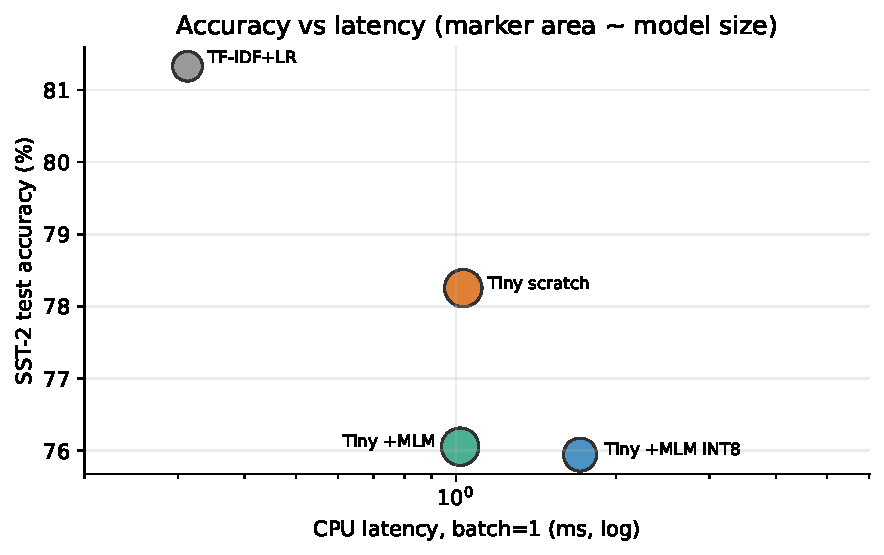
\includegraphics[width=0.7\linewidth]{fig_efficiency.pdf}
\caption{Accuracy vs.\ single-sentence CPU latency (marker area proportional to model size).}
\label{fig:eff}
\end{figure}

\subsection{RQ5: public pre-trained checkpoints}\label{sec:hf}
Table~\ref{tab:hf} and Fig.~\ref{fig:hf} add two public checkpoints under the same protocol. BERT-Tiny, whose transformer stack has the same depth and width as ours, is far better than our pre-trained model at small $n$:
$75.0\pm2.0\%$ at $n=1000$ (vs.\ $65.7\%$ ours pre-trained, $68.2\%$ ours random init, $70.5\%$ TF-IDF LogReg) and $81.7\%$ at $n=6920$, on par with TF-IDF (81.3\%) and 3--4 points above our models.
DistilBERT is best by a wide margin: $86.5\pm0.9\%$ and $90.4\pm0.2\%$, i.e.\ +16 and +9 points over TF-IDF. Pre-training therefore \emph{does} help decisively, but only with far more pre-training than we could run here.
The picture for robustness is more mixed: at $n=6920$, 30\% typos cost BERT-Tiny 7.1 and DistilBERT 6.5 points (vs.\ 3.8 for TF-IDF LogReg), and 20\% word-dropping costs 2.8 and 4.9 points.
Out of domain, neither public model beats TF-IDF: BERT-Tiny obtains $68.3$/$69.1\%$ and DistilBERT $69.0\pm6.3$/$72.8\pm1.6\%$ (at $n=1000$/$6920$) against $67.9$--$69.7$ / $72.5$--$75.5\%$ for TF-IDF, and DistilBERT's OOD accuracy varies by up to 15 points across seeds at $n=1000$ (60.5, 75.5, 71.0\%).
Confidence intervals for public vs.\ TF-IDF differences were not computed because predictions of these runs were not retained.

\begin{table}[t]
\centering\small
\caption{Public pre-trained compact checkpoints fine-tuned with the same protocol (accuracy \%, mean$\pm$std over the seeds run).}\label{tab:hf}
\resizebox{\linewidth}{!}{\begin{tabular}{lcccccc}
\toprule
Checkpoint & Params (M) & $n$ & Clean & typos 30\% & word-drop 20\% & OOD IMDb \\
\midrule
bert\_uncased\_L-2\_H-128\_A-2 & 4.4 & 1000 & 75.0$\pm$2.0 & 70.3$\pm$0.6 & 72.4$\pm$1.9 & 68.3$\pm$0.6 \\
bert\_uncased\_L-2\_H-128\_A-2 & 4.4 & 6920 & 81.7$\pm$0.0 & 74.6$\pm$0.5 & 78.9$\pm$0.2 & 69.1$\pm$1.4 \\
distilbert-base-uncased & 66.4 & 1000 & 86.5$\pm$0.9 & 80.5$\pm$0.6 & 82.4$\pm$1.6 & 69.0$\pm$6.3 \\
distilbert-base-uncased & 66.4 & 6920 & 90.4$\pm$0.2 & 83.9$\pm$0.3 & 85.5$\pm$0.1 & 72.8$\pm$1.6 \\
\bottomrule
\end{tabular}}
\end{table}

% Optional (appear after running hf_benchmark.py for more models and make_assets.py):
\IfFileExists{tables/tab_hf_eff.tex}{\input{tables/tab_hf_eff.tex}}{}
\IfFileExists{tables/tab_hf_stats.tex}{\input{tables/tab_hf_stats.tex}}{}

\begin{figure}[t]
\centering
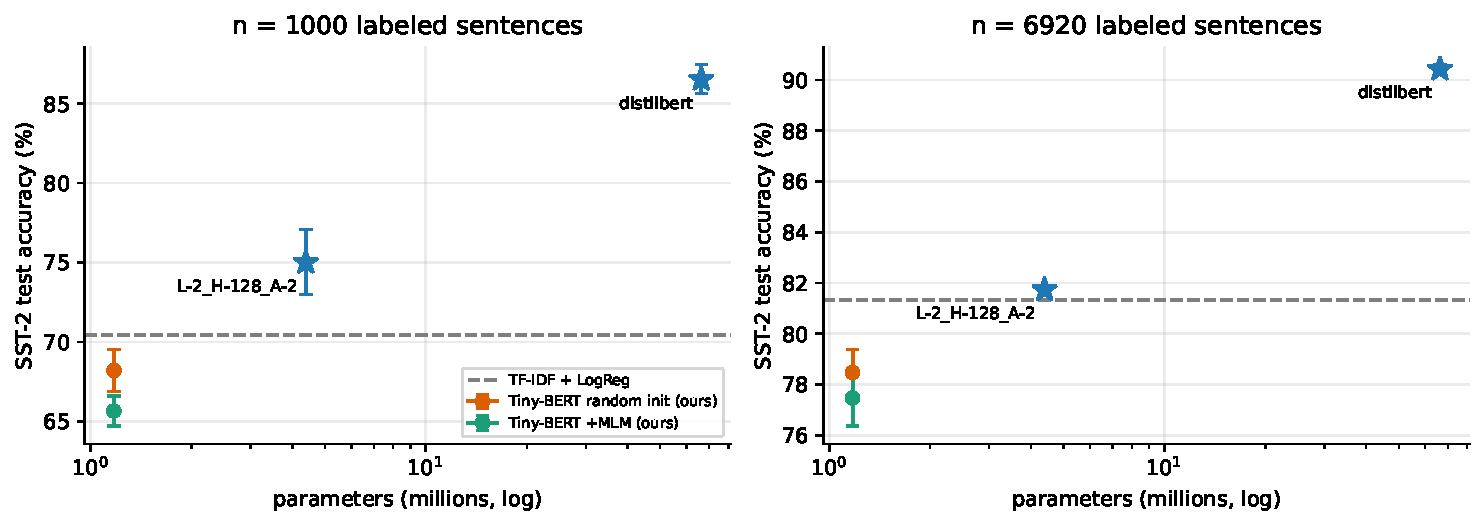
\includegraphics[width=\linewidth]{fig_hf.pdf}
\caption{SST-2 accuracy vs.\ parameter count for our tiny BERTs, the public checkpoints (stars) and TF-IDF (dashed line); error bars are 1 std over seeds.}
\label{fig:hf}
\end{figure}

\subsection{RQ6: model families and ways of using the same text}\label{sec:families}
Table~\ref{tab:families} and Fig.~\ref{fig:families} compare families under one protocol. Three patterns stand out.

\emph{The best use of unlabeled text depends on the label budget.} fastText trained on our 1.2\,M unlabeled words has the highest mean accuracy of all models at 100 and 300 labels ($60.2\%$ and $66.4\%$ vs.\ $58.6\%$ and $65.1\%$ for the best TF-IDF variant), is $4.5$ points above MLM pre-training at $n{=}1000$ ($70.2\%$ vs.\ $65.7\%$) and $2.0$ above random init ($68.2\%$), but then plateaus ($70.7\%$ at 3\,000, $71.2\%$ at 6\,920) while the transformers keep improving ($75.2$--$78.5\%$ and $72.9$--$77.5\%$). The crossover with the transformers lies between 1\,000 and 3\,000 labels.
The stratified bootstrap of Section~\ref{sec:ambiguity} agrees: at $n{=}1000$, +MLM trails fastText on strong ($-6.0$ [$-9.1$,$-2.9$]) and weak ($-3.6$ [$-6.3$,$-0.9$]) sentences, while at $n{=}6920$ it is ahead by $+5.7$ and $+6.6$ points. Word2vec behaves similarly but lower ($67.2\%$ and $68.6\%$); the sub-word model is $\approx3$ points better.
The static families are cheap: training took under one second per run (excluding a one-off embedding fit).

\emph{A lexicon with no task labels is a strong anchor.} VADER reaches $69.4\%$ with zero task labels, more than both of our transformers with 1\,000 labels ($68.2\%$, $65.7\%$) and equivalent to about 840 TF-IDF labels (Table~\ref{tab:equiv}). It is the least robust out of domain ($59.8\%$), which is unsurprising for a lexicon built for social-media text.

\emph{Character n-grams buy typo robustness.} They give the best classical accuracy at $n{=}1000$ ($71.9\%$) and $78.7\%$ under 30\% typos at $n{=}6920$ (a 2.8-point drop vs.\ 3.8 for word TF-IDF and 7.1 for BERT-Tiny), but are weaker out of domain ($70.8\%$ vs.\ $72.5$--$75.5\%$). A linear SVM on word TF-IDF is indistinguishable from logistic regression ($70.5\%$, $80.5\%$).

\begin{table}[t]
\centering\small
\caption{Model families under one protocol (accuracy \%, mean$\pm$std over 3 seeds; VADER uses no task labels, so its row is independent of $n$; robustness columns at $n{=}6920$).}\label{tab:families}
\resizebox{\linewidth}{!}{\begin{tabular}{lccccc}
\toprule
Model family & $n{=}1000$ & $n{=}6920$ & 30\% typos & 20\% drop & OOD IMDb \\
\midrule
VADER lexicon (no task labels) & 69.4$\pm$0.0 & 69.4$\pm$0.0 & 66.4$\pm$0.0 & 67.2$\pm$0.0 & 59.8$\pm$0.0 \\
TF-IDF + LogReg & 70.5$\pm$0.7 & 81.3$\pm$0.0 & 77.5$\pm$0.0 & 77.9$\pm$0.0 & 72.5$\pm$0.0 \\
TF-IDF + NaiveBayes & 71.6$\pm$0.7 & 81.9$\pm$0.0 & 79.1$\pm$0.0 & 79.0$\pm$0.0 & 75.5$\pm$0.0 \\
TF-IDF word + SVM & 70.5$\pm$0.7 & 80.5$\pm$0.0 & 77.2$\pm$0.0 & 77.2$\pm$0.0 & 73.2$\pm$0.0 \\
TF-IDF char n-gram + LogReg & 71.9$\pm$0.8 & 81.5$\pm$0.0 & 78.7$\pm$0.0 & 78.4$\pm$0.0 & 70.8$\pm$0.0 \\
word2vec (same 1.2M words) + LogReg & 67.2$\pm$0.3 & 68.6$\pm$0.0 & 67.8$\pm$0.0 & 68.7$\pm$0.0 & 67.0$\pm$0.0 \\
fastText (same 1.2M words) + LogReg & 70.2$\pm$0.6 & 71.2$\pm$0.0 & 69.6$\pm$0.0 & 69.6$\pm$0.0 & 66.2$\pm$0.0 \\
Tiny-BERT (random init) & 68.2$\pm$1.3 & 78.5$\pm$0.9 & 73.6$\pm$0.8 & 77.0$\pm$0.4 & 68.1$\pm$0.7 \\
Tiny-BERT (+MLM pre-training) & 65.7$\pm$0.9 & 77.5$\pm$1.1 & 70.6$\pm$1.9 & 76.8$\pm$1.3 & 63.7$\pm$1.4 \\
\bottomrule
\end{tabular}}
\end{table}

\begin{table}[t]
\centering\small
\caption{Label-equivalence: number of TF-IDF+LogReg labels needed to match each model's accuracy (log-linear interpolation of the TF-IDF curve).}\label{tab:equiv}
\resizebox{\linewidth}{!}{\begin{tabular}{lcc}
\toprule
Model & $n{=}1000$ & $n{=}6920$ \\
\midrule
VADER lexicon (no task labels) & 840 & -- \\
TF-IDF + NaiveBayes & 1,190 & $>$6,920 \\
TF-IDF word + SVM & 1,010 & 5,720 \\
TF-IDF char n-gram + LogReg & 1,260 & $>$6,920 \\
word2vec (same 1.2M words) + LogReg & 590 & 740 \\
fastText (same 1.2M words) + LogReg & 960 & 1,120 \\
Tiny-BERT (random init) & 690 & 3,730 \\
Tiny-BERT (+MLM pre-training) & 450 & 3,000 \\
bert\_uncased\_L-2\_H-128\_A-2 & 2,040 & $>$6,920 \\
distilbert-base-uncased & $>$6,920 & $>$6,920 \\
\bottomrule
\end{tabular}}
\end{table}


\begin{figure}[t]
\centering
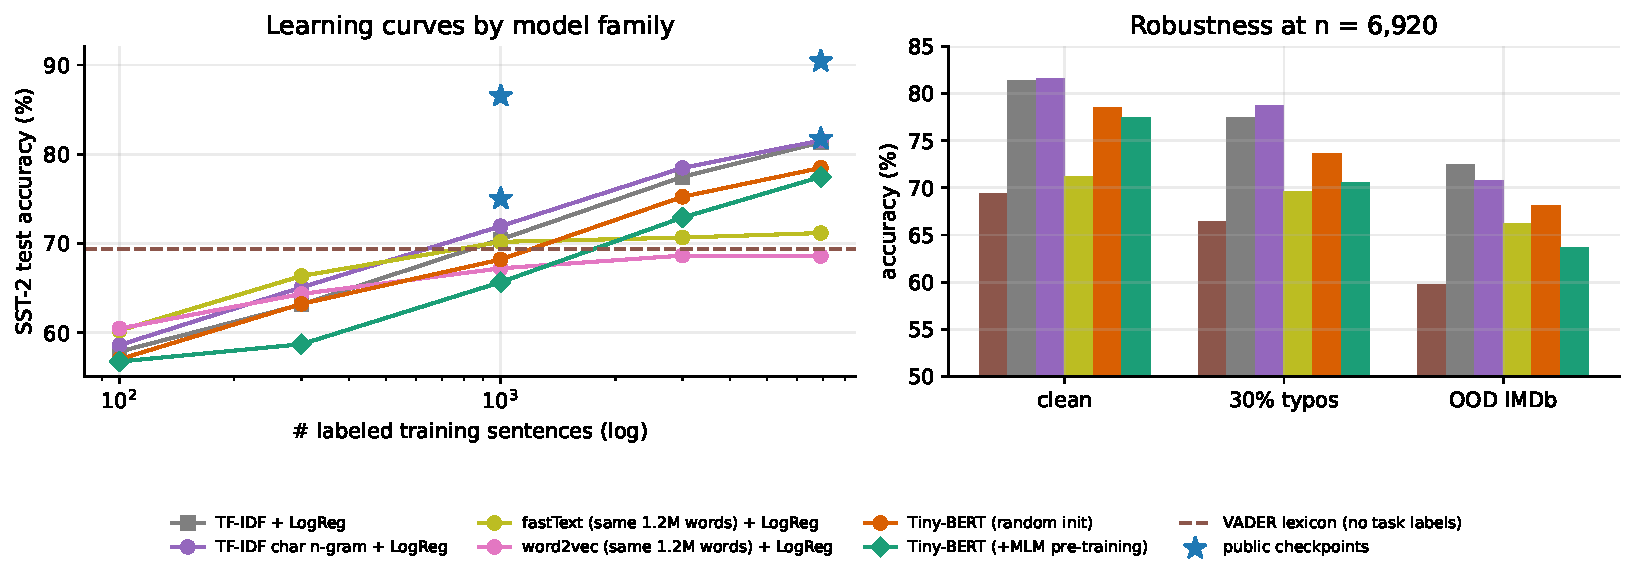
\includegraphics[width=\linewidth]{fig_families.pdf}
\caption{Model families. Left: learning curves (stars: public checkpoints at $n{=}1000$ and $6920$; dashed line: VADER, independent of $n$). Right: clean, 30\%-typo and out-of-domain accuracy at $n{=}6920$ (VADER at its label-free accuracy); bar colours as in the legend.}
\label{fig:families}
\end{figure}

\subsection{RQ7: ambiguity}\label{sec:ambiguity}
\paragraph{Does the proxy mean anything?} Sentences that few of the 27 core runs classify correctly are mostly weakly polar: $79.6\%$ ($n{=}1000$) and $81.5\%$ ($n{=}6920$) of the ``hard'' group are weak, versus $62.8\%$ overall and $55.4\%$--$56.7\%$ of the ``easy'' group (Table~\ref{tab:ambvalid}); the Spearman correlation between consensus difficulty and polarity strength is $0.21$ and $0.23$. The proxy is thus modestly but consistently related to what is hard for models.

\paragraph{Everyone struggles with weak polarity.} All models are 8--13 points less accurate on weak than on strong sentences (Tables~\ref{tab:amb1000}, \ref{tab:amb6920}; Fig.~\ref{fig:ambiguity}).

\paragraph{Where the pre-training deficit lies.} At $n{=}1000$ the MLM-pre-trained model is worse than its random-init twin by $4.7$ points on strong sentences ($[-7.2,-2.2]$) but only $1.3$ on weak ones ($[-3.4,+0.8]$, includes 0); the interaction, $-3.5$ [$-6.7$,$-0.3$], excludes zero (Table~\ref{tab:ambci}). At $n{=}6920$ the pattern is the same ($-2.6$ [$-4.8$,$-0.2$] vs.\ $-0.1$ [$-2.2$,$+1.9$]) but the interaction, $-2.4$ [$-5.6$,$+0.4$], is not resolved. Pre-training therefore lost mainly on \emph{clearly} polar sentences, where sparse lexical cues suffice, and roughly tied on ambiguous ones.

\paragraph{Contrast and negation.} Contrast words occur in 18.5\% of the sentences and 76.3\% of those are weakly polar (59.7\% otherwise). Every model is less accurate on them at $n{=}6920$: TF-IDF LR $75.4\%$ vs.\ $82.7\%$, random init $75.3\%$ vs.\ $79.2\%$, +MLM $74.1\%$ vs.\ $78.2\%$, character LR $78.0\%$ vs.\ $82.3\%$, and the bag-of-embeddings fastText model $65.0\%$ vs.\ $72.6\%$.
The from-scratch transformer \emph{ties} TF-IDF on contrast sentences ($-0.1$ [$-4.3$,$+3.9$]) while trailing it on all others ($-3.5$ [$-5.4$,$-1.6$]), and it beats fastText on contrast sentences by $+10.3$ [$+5.3$,$+15.0$] points (vs.\ $+6.6$ elsewhere). This is consistent with contextual models coping better with compositional sentences, but the intervals for the contrast stratum are wide and we did not test the difference between strata.

\paragraph{Do confidences reflect ambiguity?} Barely. The ambiguity-awareness AUROC ranges from $0.545$ to $0.622$ (chance: 0.5): highest for character LR ($0.622$) and word LR ($0.617$) at $n{=}6920$, $0.604$ for both transformers, and $0.553$--$0.559$ for the lexicon and static embeddings; pre-training does not improve it ($0.604$ vs.\ $0.604$ at $n{=}6920$; $0.545$ vs.\ $0.561$ at $n{=}1000$).
At $n{=}1000$ the random-init transformer's mean confidence is $0.943$ on strong and $0.931$ on weak sentences (gap $0.012$) against $0.719$ vs.\ $0.683$ (gap $0.036$) for TF-IDF LR. Calibration is far worse for the transformers at small $n$ (ECE $25.6\%$ random init, $22.9\%$ pre-trained vs.\ $3.1$--$6.4\%$ for TF-IDF, character and static models), improving to $8.2\%$ and $7.6\%$ at $n{=}6920$ (others $2.8$--$5.1\%$).
Consequently, an abstention rule that keeps the 50\% most confident predictions is more accurate for TF-IDF ($82.2\%$ at $n{=}1000$, $94.0\%$ at $n{=}6920$) than for the transformers ($78.8/74.8\%$ and $91.6/89.3\%$). The public checkpoints are not part of this analysis because predictions were not stored for the earlier runs (\texttt{hf\_benchmark.py --rerun} regenerates them).

\begin{table}[t]
\centering\small
\caption{Convergent validity of the polarity-strength proxy: share of weak-polarity sentences among those that few/many of the 27 model runs classify correctly.}\label{tab:ambvalid}
\resizebox{\linewidth}{!}{\begin{tabular}{llcc}
\toprule
$n$ & Consensus difficulty group & Sentences & Share weak polarity \\
\midrule
1000 & hard ($<$25\% of runs correct) & 98 & 79.6\% \\
1000 & middle & 846 & 68.4\% \\
1000 & easy ($\geq$75\% correct) & 877 & 55.4\% \\
1000 & all sentences (base rate) & 1821 & 62.8\% \\
6920 & hard ($<$25\% of runs correct) & 124 & 81.5\% \\
6920 & middle & 490 & 73.1\% \\
6920 & easy ($\geq$75\% correct) & 1207 & 56.7\% \\
6920 & all sentences (base rate) & 1821 & 62.8\% \\
\bottomrule
\end{tabular}}
\end{table}

\begin{table}[t]
\centering\small
\caption{Accuracy (\%) on strong- vs weak-polarity sentences, ambiguity-awareness AUROC (0.5 = chance), calibration error (ECE, \%; -- for score-only models) and accuracy on the 50\% most confident predictions; $n=1000$ labels, mean over 3 seeds (strong: 678 sentences, weak: 1\,143).}\label{tab:amb1000}
\resizebox{\linewidth}{!}{\begin{tabular}{lcccccc}
\toprule
Model & Acc.\ strong & Acc.\ weak & Gap & Ambiguity AUROC & ECE & Acc.@50\% cov. \\
\midrule
TF-IDF + LogReg & 77.3 & 66.4 & 10.9 & 0.582 & 3.1 & 82.2 \\
TF-IDF char n-gram + LogReg & 79.8 & 67.3 & 12.5 & 0.579 & 6.4 & 83.4 \\
TF-IDF word + SVM & 77.3 & 66.6 & 10.7 & 0.581 & -- & 82.2 \\
VADER lexicon (no task labels) & 77.4 & 64.7 & 12.8 & 0.559 & -- & 78.5 \\
fastText (same 1.2M words) + LogReg & 75.0 & 67.3 & 7.6 & 0.552 & 5.5 & 81.0 \\
word2vec (same 1.2M words) + LogReg & 72.2 & 64.2 & 8.0 & 0.545 & 4.8 & 79.2 \\
Tiny-BERT (random init) & 73.6 & 65.0 & 8.7 & 0.561 & 25.6 & 78.8 \\
Tiny-BERT (+MLM pre-training) & 68.9 & 63.7 & 5.2 & 0.545 & 22.9 & 74.8 \\
\bottomrule
\end{tabular}}
\end{table}

\begin{table}[t]
\centering\small
\caption{Accuracy (\%) on strong- vs weak-polarity sentences, ambiguity-awareness AUROC (0.5 = chance), calibration error (ECE, \%; -- for score-only models) and accuracy on the 50\% most confident predictions; $n=6920$ labels, mean over 3 seeds (strong: 678 sentences, weak: 1\,143).}\label{tab:amb6920}
\resizebox{\linewidth}{!}{\begin{tabular}{lcccccc}
\toprule
Model & Acc.\ strong & Acc.\ weak & Gap & Ambiguity AUROC & ECE & Acc.@50\% cov. \\
\midrule
TF-IDF + LogReg & 88.1 & 77.3 & 10.7 & 0.617 & 4.4 & 94.0 \\
TF-IDF char n-gram + LogReg & 88.9 & 77.2 & 11.8 & 0.622 & 2.8 & 92.3 \\
TF-IDF word + SVM & 87.8 & 76.1 & 11.6 & 0.611 & -- & 93.6 \\
VADER lexicon (no task labels) & 77.4 & 64.7 & 12.8 & 0.559 & -- & 78.5 \\
fastText (same 1.2M words) + LogReg & 77.4 & 67.5 & 10.0 & 0.553 & 3.2 & 84.2 \\
word2vec (same 1.2M words) + LogReg & 75.5 & 64.5 & 11.0 & 0.554 & 3.7 & 81.9 \\
Tiny-BERT (random init) & 85.7 & 74.2 & 11.5 & 0.604 & 8.2 & 91.6 \\
Tiny-BERT (+MLM pre-training) & 83.1 & 74.1 & 9.0 & 0.604 & 7.6 & 89.3 \\
\bottomrule
\end{tabular}}
\end{table}

\begin{table}[t]
\centering\small
\caption{Paired bootstrap (95\% CI, points) of accuracy differences within ambiguity strata; ``Strong$-$weak'' tests whether the difference is larger on strong than on weak sentences. $^*$ = CI excludes 0.}\label{tab:ambci}
\resizebox{\linewidth}{!}{\begin{tabular}{llccccc}
\toprule
$n$ & Comparison & Strong & Weak & Strong$-$weak & Contrast & No contrast \\
\midrule
1000 & +MLM $-$ random init & -4.7 [-7.2, -2.2]$^*$ & -1.3 [-3.4, +0.8] & -3.5 [-6.7, -0.3]$^*$ & -4.1 [-8.1, +0.2] & -2.2 [-4.0, -0.4]$^*$ \\
1000 & +MLM $-$ TF-IDF LR & -8.4 [-11.3, -5.6]$^*$ & -2.7 [-5.0, -0.4]$^*$ & -5.7 [-9.3, -2.1]$^*$ & -4.9 [-9.2, -0.3]$^*$ & -4.8 [-6.8, -2.8]$^*$ \\
1000 & random init $-$ TF-IDF LR & -3.6 [-5.8, -1.3]$^*$ & -1.4 [-3.4, +0.4] & -2.2 [-5.1, +0.6] & -0.9 [-4.1, +2.5] & -2.6 [-4.1, -1.0]$^*$ \\
1000 & random init $-$ fastText & -1.3 [-4.3, +1.8] & -2.4 [-4.8, +0.1] & +1.0 [-2.8, +4.8] & +2.7 [-1.7, +7.0] & -3.0 [-5.1, -0.9]$^*$ \\
1000 & +MLM $-$ fastText & -6.0 [-9.1, -2.9]$^*$ & -3.6 [-6.3, -0.9]$^*$ & -2.4 [-6.3, +1.5] & -1.4 [-6.2, +3.8] & -5.2 [-7.4, -2.9]$^*$ \\
6920 & +MLM $-$ random init & -2.6 [-4.8, -0.2]$^*$ & -0.1 [-2.2, +2.0] & -2.5 [-5.6, +0.3] & -1.2 [-4.8, +2.7] & -1.0 [-2.6, +0.6] \\
6920 & +MLM $-$ TF-IDF LR & -4.9 [-7.6, -2.4]$^*$ & -3.2 [-5.8, -0.6]$^*$ & -1.7 [-5.4, +2.0] & -1.3 [-6.0, +3.7] & -4.4 [-6.4, -2.4]$^*$ \\
6920 & random init $-$ TF-IDF LR & -2.4 [-4.7, -0.0]$^*$ & -3.1 [-5.6, -0.8]$^*$ & +0.8 [-2.5, +4.0] & -0.1 [-4.3, +3.9] & -3.5 [-5.4, -1.6]$^*$ \\
6920 & random init $-$ fastText & +8.3 [+5.1, +11.6]$^*$ & +6.7 [+4.0, +9.7]$^*$ & +1.5 [-2.6, +5.7] & +10.3 [+5.3, +15.0]$^*$ & +6.6 [+4.2, +9.0]$^*$ \\
6920 & +MLM $-$ fastText & +5.7 [+2.4, +9.0]$^*$ & +6.6 [+3.9, +9.5]$^*$ & -0.9 [-5.3, +3.3] & +9.1 [+3.8, +14.3]$^*$ & +5.7 [+3.3, +8.0]$^*$ \\
\bottomrule
\end{tabular}}
\end{table}


\begin{figure}[t]
\centering
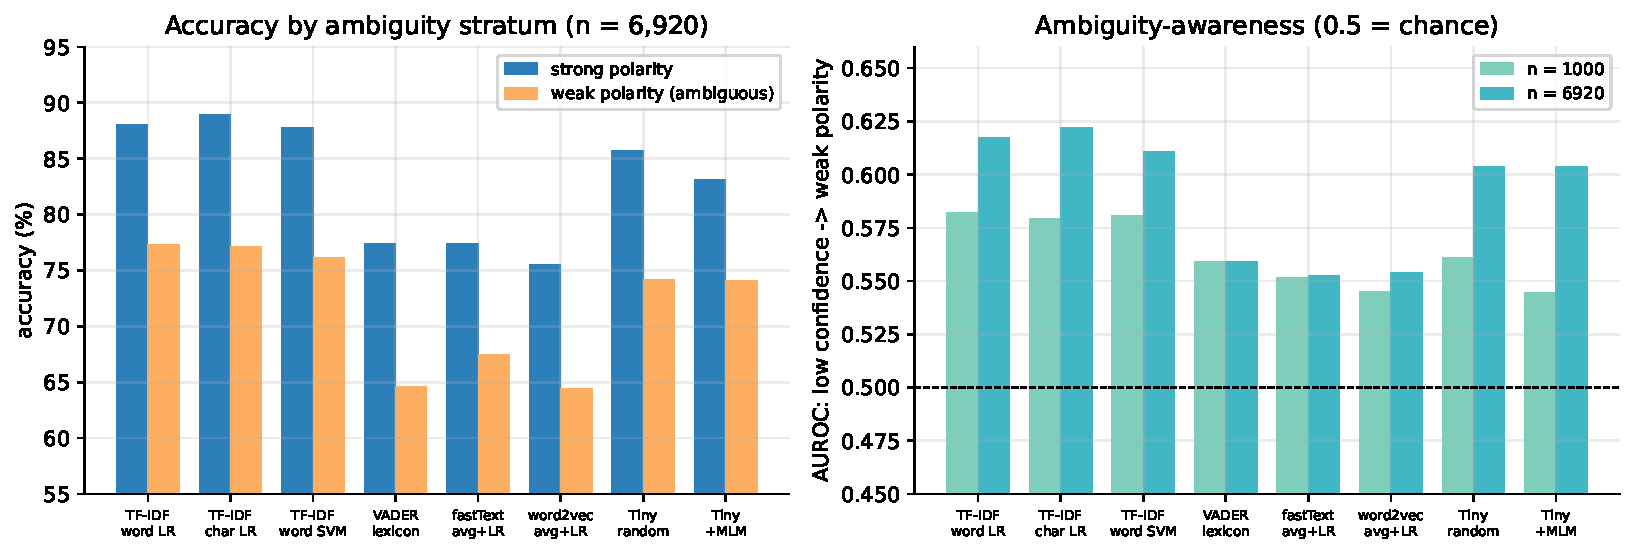
\includegraphics[width=\linewidth]{fig_ambiguity.pdf}
\caption{Ambiguity. Left: accuracy on strong- vs.\ weak-polarity sentences at $n{=}6920$. Right: ambiguity-awareness AUROC (how well low confidence identifies weak-polarity sentences; dashed line = chance).}
\label{fig:ambiguity}
\end{figure}

\begin{table}[t]
\centering\small
\caption{Learning-rate pilot: dev accuracy (\%) (seed 0). The rate with the best mean over the two sizes is used in all later experiments.}\label{tab:pilot}
\resizebox{\linewidth}{!}{\begin{tabular}{lcccccc}
\toprule
Model & $n$ & 2e-4 & 5e-4 & 1e-3 & 2e-3 & 4e-3 \\
\midrule
Tiny-BERT (random init) & 300 & 63.3 & 63.5 & 63.3 & 62.3 & 63.0 \\
Tiny-BERT (random init) & 3000 & 76.3 & 74.7 & 74.3 & 72.8 & 70.5 \\
Tiny-BERT (+MLM pre-training) & 300 & 63.0 & 62.0 & 61.6 & 62.0 & 59.2 \\
Tiny-BERT (+MLM pre-training) & 3000 & 74.2 & 74.8 & 74.8 & 71.7 & 62.6 \\
\bottomrule
\end{tabular}}
\end{table}


\subsection{RQ8: cross-domain generalisation}\label{sec:crossdomain}
\paragraph{Do the RQ1/RQ6 findings replicate?} Table~\ref{tab:fin_air} gives the learning curves for both new domains. In finance, MLM pre-training does \emph{not} beat random init at any budget (e.g.\ $69.8\pm1.4\%$ vs.\ $70.2\pm3.3\%$ at $n{=}50$; $86.3\pm1.2\%$ vs.\ $87.2\pm1.0\%$ at $n{=}1377$), matching the SST-2 pattern. In airline, the same holds at small $n$ and the effect is significant: at $n{=}100$, +MLM trails random init by $-1.9$ points ($95\%$ CI $[-2.5,-1.2]$, excludes zero), and fastText beats +MLM by $+3.2$ points ($[+2.3,+4.1]$) -- both replicate the RQ1/RQ6 story that at small budgets a cheaper use of the same (or no) unlabeled text beats contextual pre-training.
\emph{Unlike SST-2}, at full data all three families become statistically indistinguishable in the new domains: the paired bootstrap for +MLM vs.\ random init, +MLM vs.\ TF-IDF, and random init vs.\ TF-IDF all have intervals that include zero at $n{=}1377$ (finance) and $n{=}8125$ (airline), whereas on SST-2 TF-IDF still leads +MLM by $-3.9$ points (CI excludes zero) at $n{=}6920$. One plausible reason is that finance and airline are more lexicon-driven (sentiment words like ``profit'' or ``delay'' carry more of the signal) so all methods converge with enough labels; we did not test this directly.
Class balance differs sharply by domain (SST-2 $\approx$50/50, finance 69\% positive, airline 80\% negative), so Table~\ref{tab:fin_air} should be read alongside macro-F1 (\texttt{results/all\_runs.csv}) rather than accuracy alone for the more imbalanced airline domain.

\begin{table}[t]
\centering\small\setlength{\tabcolsep}{3pt}
\caption{Finance (top; $n=50,100,300,700,1377$) and Airline (bottom; $n=100,300,1000,3000,8125$) learning curves, test accuracy (\%), mean$\pm$std over 3 seeds.}\label{tab:fin_air}
\begin{tabular}{lccccc}
\toprule
Model & $n_1$ & $n_2$ & $n_3$ & $n_4$ & $n_5$ (full) \\
\midrule
TF-IDF + LogReg & 71.7$\pm$1.0 & 73.7$\pm$1.7 & 79.3$\pm$0.6 & 84.6$\pm$1.4 & 87.3$\pm$0.0 \\
TF-IDF + NaiveBayes & 72.3$\pm$1.2 & 74.8$\pm$1.9 & 79.2$\pm$0.9 & 85.2$\pm$1.1 & 83.2$\pm$0.0 \\
Tiny-BERT random init & 68.9$\pm$1.6 & 72.8$\pm$2.5 & 80.9$\pm$1.1 & 86.5$\pm$0.2 & 87.2$\pm$1.0 \\
Tiny-BERT +MLM & 69.5$\pm$0.2 & 70.0$\pm$1.2 & 77.4$\pm$1.9 & 83.7$\pm$1.2 & 86.5$\pm$1.1 \\
\midrule
TF-IDF + LogReg & 83.5$\pm$1.5 & 85.9$\pm$0.3 & 88.1$\pm$0.3 & 90.1$\pm$0.1 & 92.0$\pm$0.0 \\
TF-IDF + NaiveBayes & 84.1$\pm$1.2 & 84.7$\pm$0.4 & 86.1$\pm$0.2 & 87.6$\pm$0.1 & 89.2$\pm$0.0 \\
Tiny-BERT random init & 84.4$\pm$1.0 & 85.5$\pm$0.4 & 88.1$\pm$0.8 & 90.9$\pm$0.4 & 91.6$\pm$0.2 \\
Tiny-BERT +MLM & 82.6$\pm$0.5 & 83.7$\pm$0.9 & 87.1$\pm$0.3 & 89.6$\pm$0.3 & 91.5$\pm$0.5 \\
\midrule
\bottomrule
\end{tabular}
\end{table}

\begin{table}[t]
\centering\small
\caption{Cross-domain transfer: full-data models evaluated on their own and the other two domains' test sets (single seed-0 run per cell unless otherwise noted).}\label{tab:cross}
\resizebox{\linewidth}{!}{\begin{tabular}{llll}
\toprule
Model & Trained on & Tested on & Accuracy (\%) \\
\midrule
Tiny-BERT (+MLM pre-training) & SST-2 (movies) & SST-2 (movies) & 77.5 \\
Tiny-BERT (+MLM pre-training) & SST-2 (movies) & Finance (news) & 51.8 \\
Tiny-BERT (+MLM pre-training) & SST-2 (movies) & Airline (tweets) & 68.3 \\
Tiny-BERT (+MLM pre-training) & Finance (news) & SST-2 (movies) & 54.1 \\
Tiny-BERT (+MLM pre-training) & Finance (news) & Finance (news) & 86.5 \\
Tiny-BERT (+MLM pre-training) & Finance (news) & Airline (tweets) & 47.2 \\
Tiny-BERT (+MLM pre-training) & Airline (tweets) & SST-2 (movies) & 55.6 \\
Tiny-BERT (+MLM pre-training) & Airline (tweets) & Finance (news) & 33.4 \\
Tiny-BERT (+MLM pre-training) & Airline (tweets) & Airline (tweets) & 91.5 \\
Tiny-BERT (random init) & SST-2 (movies) & SST-2 (movies) & 78.5 \\
Tiny-BERT (random init) & SST-2 (movies) & Finance (news) & 52.3 \\
Tiny-BERT (random init) & SST-2 (movies) & Airline (tweets) & 73.8 \\
Tiny-BERT (random init) & Finance (news) & SST-2 (movies) & 53.0 \\
Tiny-BERT (random init) & Finance (news) & Finance (news) & 87.2 \\
Tiny-BERT (random init) & Finance (news) & Airline (tweets) & 35.6 \\
Tiny-BERT (random init) & Airline (tweets) & SST-2 (movies) & 56.5 \\
Tiny-BERT (random init) & Airline (tweets) & Finance (news) & 35.4 \\
Tiny-BERT (random init) & Airline (tweets) & Airline (tweets) & 91.6 \\
TF-IDF + LogReg & SST-2 (movies) & SST-2 (movies) & 81.3 \\
TF-IDF + LogReg & SST-2 (movies) & Finance (news) & 62.7 \\
TF-IDF + LogReg & SST-2 (movies) & Airline (tweets) & 75.3 \\
TF-IDF + LogReg & Finance (news) & SST-2 (movies) & 52.2 \\
TF-IDF + LogReg & Finance (news) & Finance (news) & 87.3 \\
TF-IDF + LogReg & Finance (news) & Airline (tweets) & 26.8 \\
TF-IDF + LogReg & Airline (tweets) & SST-2 (movies) & 53.0 \\
TF-IDF + LogReg & Airline (tweets) & Finance (news) & 32.0 \\
TF-IDF + LogReg & Airline (tweets) & Airline (tweets) & 92.0 \\
\bottomrule
\end{tabular}}
\end{table}


\paragraph{Cross-domain transfer.} Table~\ref{tab:cross} and Fig.~\ref{fig:cross} evaluate every full-data model, zero-shot, on the other two domains. Every model loses 15--60 points off its in-domain accuracy when moved to a different domain. TF-IDF trained on SST-2 transfers best (62.7\% on finance, 75.3\% on airline) -- better than either tiny transformer trained on the same data (51.8--56.5\%), consistent with Section~\ref{sec:families}'s finding that sparse lexical features generalise more predictably than a small transformer's learned representation.
Transfer \emph{into} finance and airline from each other is the weakest cell in the matrix (26.8--35.6\%, often below the 50\% chance rate for a balanced problem): a model trained on finance's 69\%-positive text, applied to airline's 80\%-negative tweets, is biased toward the wrong class before it even sees the input's content -- a base-rate mismatch compounding the vocabulary mismatch. MLM pre-training does not reduce this transfer gap: the pre-trained model is within 1--3 points of its random-init twin in every off-diagonal cell.

\begin{figure}[t]
\centering
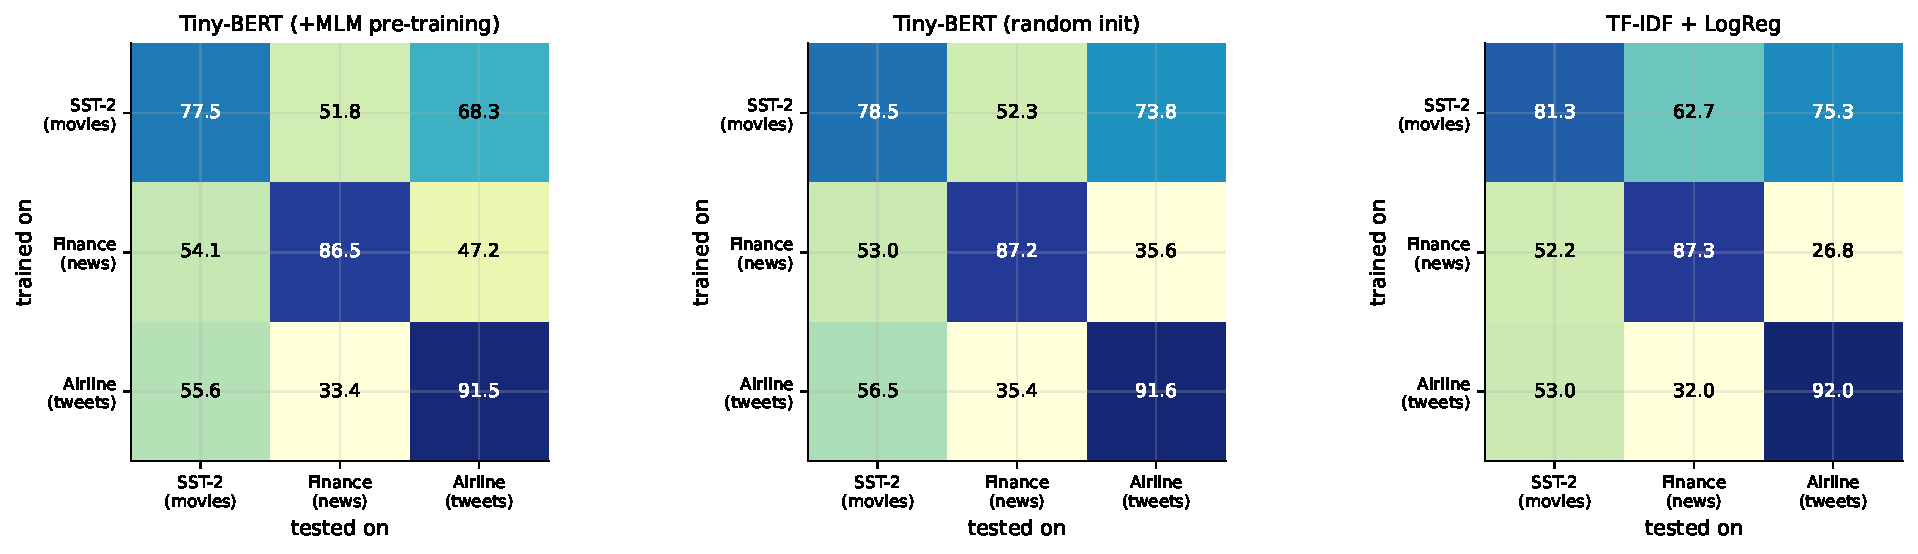
\includegraphics[width=\linewidth]{fig_cross_domain.pdf}
\caption{Cross-domain transfer matrix: full-data (seed-0) models trained on one domain (rows), tested on all three (columns). Diagonal = in-domain.}
\label{fig:cross}
\end{figure}

\section{Discussion}
\textbf{Same words, different bets.} Given 1.2\,M unlabeled words, three bets are possible: ignore them (TF-IDF, lexicon), distil them into static vectors (word2vec/fastText), or learn a contextual model by MLM. Our data say the best bet depends on the label budget: static vectors win with a few hundred labels, sparse features and from-scratch transformers win later, and contextual pre-training at this scale never came out ahead.
A lexicon with no task labels is already worth about 840 labels, which puts the ``cost'' of the neural options in perspective.

\textbf{Why did our pre-training not help?} The evidence points at scale rather than architecture: BERT-Tiny shares our depth and width yet gains 7--9 points at $n=1000$ over our models, and it was pre-trained by its authors \cite{turc2019well} on a much larger corpus, with a larger vocabulary that we cannot separate from data scale.
Plausible contributors are the tiny corpus and compute (final masked accuracy 29\%), the domain gap between long IMDb reviews and short critic snippets, and the limited capacity of a 1.17\,M-parameter model. The decoupling between a rising frozen-probe accuracy and a falling fine-tuned accuracy suggests that our pre-trained weights are a better representation but a worse starting point at a fixed small learning rate; both learning-rate pilots chose the lowest grid value, so better-tuned optimisation might change the size of the gap. We did not test these explanations.

\textbf{What ambiguity adds.} The loss from pre-training is concentrated where sentiment is unambiguous, while on ambiguous sentences it is close to a tie; transformers cope relatively well with contrast sentences; and no family is good at knowing when it faces an ambiguous sentence (AUROC $\le0.62$), with the transformers additionally over-confident when trained on few labels.
For deployment this suggests that raw confidences of small fine-tuned transformers should not be used to flag ambiguous inputs without recalibration, and that TF-IDF-style models give more trustworthy abstention at small $n$.

\textbf{Practical guidance.} With a CPU, a few hundred labels and unlabeled in-domain text: fastText features; with a few thousand: TF-IDF (word or character) or a from-scratch transformer that is no better; with a public checkpoint: BERT-Tiny matches TF-IDF at full data and is about twice as label-efficient at 1\,000 labels, and DistilBERT is decisively better but takes about 26 minutes to fine-tune here. Character n-grams for noisy text. Do not trust small-$n$ transformer confidences.

\textbf{Does any of this generalise?} Extending RQ1 and RQ6 to finance news and airline tweets replicates the low-budget story (fastText/cheaper features beat MLM pre-training) but not the full-data story: on SST-2, TF-IDF keeps a significant edge even at 6\,920 labels, while in the two new domains all three families converge to statistical ties by their full budgets. And no model, including the pre-trained one, transfers its accuracy across domains: cross-domain accuracy drops by 15--60 points, and the drop is dominated by vocabulary and base-rate mismatch rather than by anything pre-training fixes.

\subsection*{Limitations}
\begin{itemize}
\item \textbf{One task, one dataset, one language} (SST-2 sentiment in English, with IMDb reviews as the only shift). Conclusions about model families and ambiguity may not transfer.
\item \textbf{Ambiguity proxies.} Polarity strength (SST-5) measures intensity, not annotator disagreement; ``weak'' covers 62.8\% of sentences; the linguistic markers are crude. The consensus signal is built from the same models it is used to analyse, so it only serves as a validity check.
\item \textbf{Only two public checkpoints} (BERT-Tiny, DistilBERT) in the main results, with untuned learning rates; their predictions were not stored, so they are absent from the ambiguity/calibration analysis and from paired tests. The code supports BERT-Mini/Small/Medium, MiniLM, TinyBERT and ELECTRA-small (\texttt{hf\_benchmark.py}), but they were not run.
\item \textbf{Untuned families.} Embedding dimension, epochs and pooling (simple averaging) were fixed; CNN/BiLSTM models were not included.
\item Three seeds; full 872-sentence dev set for early stopping even at $n=100$; a learning-rate pilot with two sizes and one seed whose selected value lies at the grid edge; a small OOD set (400 documents).
\item Efficiency numbers are single-thread measurements for one model per configuration on one machine. The lightweight families and post-hoc analyses are deterministic scripts that can be regenerated in minutes.
\item \textbf{Cross-domain results use single-model (seed-0) cells for the transfer matrix} (Table~\ref{tab:cross}), not averaged over seeds, and \texttt{tfidf\_nb} was not included in the cross-domain backfill, so it is absent from the seed-complete comparisons.
\item \textbf{Finance and airline test sets are class-imbalanced} (69\% positive, 80\% negative respectively, vs.\ near-balanced SST-2); accuracy comparisons across domains should be read alongside macro-F1.
\end{itemize}

\section{Conclusion}
Given 1.2\,M unlabeled words, contextual MLM pre-training with 13 CPU-minutes was the \emph{worst} way to use them at small label budgets: it did not beat random initialisation, static fastText vectors beat it with up to 1\,000 labels, and TF-IDF variants beat it from 300 labels on.
Its deficit sits on unambiguous, strongly polar sentences; on ambiguous ones it ties. Public pre-trained checkpoints show that the picture changes with scale: BERT-Tiny matches TF-IDF at full data and DistilBERT is far ahead.
All models, transformers most of all when trained on few labels, are poor at flagging ambiguity through their confidence. Extending the study to finance news and airline tweets shows the small-budget pattern generalises (a cheaper use of unlabeled text beats pre-training) while the full-data pattern does not (TF-IDF's edge on SST-2 disappears in the new domains), and that none of the three families transfer across domains without a large accuracy cost. Natural next steps are more public checkpoints with tuned learning rates and stored predictions (so that the ambiguity analysis can be extended across a size ladder), annotator-disagreement data as a stronger ambiguity signal, and a larger in-domain corpus.

\section*{Reproducibility}
All code, logs, raw per-run results (\texttt{results/results.jsonl}, \texttt{families.jsonl}, \texttt{hf\_results.jsonl}, \texttt{all\_runs.csv}), stored predictions and the scripts generating every figure and table (\texttt{src/make\_assets.py}, \texttt{src/ambiguity.py}) are included; see \texttt{README.md}.
Logged warnings about missing \texttt{blake2} hash functions come from the Python installation and do not affect any result.

\bibliographystyle{plain}
\bibliography{refs}

\end{document}
